\titleformat{\chapter}[display]
{\normalfont\Large\BNazboldEGT\centering}
{\vspace*{8cm}{‎\textbf{فصل چهارم} }}{5pt}{\Large}
\chapter{\textbf{آزمایشات}}\label{sec4}
\thispagestyle{empty}
\newpage

\begin{table}
	\centering
	\small
	\caption{جزئیات مجموعه‌داده‌های دنیای واقعی}
	\setLTRtable
	\begin{tabular}{lcccccc}
		\hline
		مجموعه‌داده & \#نمونه & \#ویژگی & \#برچسب\\
		\hline
		\lr{Arts}       & 5000 & 462 & 26 \\
		\lr{Business}   & 5000 & 438 & 30 \\
		\lr{Computers}  & 5000 & 681 & 33 \\
		\lr{corel5k}    & 5000 & 499 & 374 \\
		\lr{Education}  & 5000 & 550 & 33 \\
		\lr{Entertainment} & 5000 & 640 & 21 \\
		\lr{Health}     & 5000 & 612 & 32 \\
		\lr{Recreation} & 5000 & 606 & 22 \\
		\lr{Reference}  & 5000 & 793 & 33 \\
		\lr{Science}    & 5000 & 743 & 40 \\
		\lr{Social}     & 5000 & 1047 & 39 \\
		\lr{Society}    & 5000 & 636 & 27 \\
		\hline
	\end{tabular}
	\label{tab:datasets}
\end{table}
این بخش یک ارزیابی جامع برای مدل ‎\lr{MLFS-GLOCAL}‎ بر روی 12 مجموعه‌داده چندبرچسبه واقعی با استفاده از شش معیار\LTRfootnote{Metric}} ارزیابی متنوع انجام می‌دهد. همچنین مدل پیشنهادی با نُه روش شناخته‌شده و پیشرفته انتخاب ویژگی مقایسه شده است.‎
\section{مجموعه‌داده‌ها}
در بخش آزمایشات، از ۱۲ مجموعه‌داده از کتابخانه \lr{Mulan} برای طبقه‌بندی متن و تصاویر چندبرچسبه استفاده شده است. مجموعه‌داده‌های چندبرچسبه یاهو\LTRfootnote{Yahoo} به مجموعه‌ای از چندین مجموعه‌داده اشاره دارد که برای طبقه‌بندی مسائل چندبرچسبه استفاده می‌شوند. این‌ داده‌ها، توسط آزمایشگاه‌های یاهو منتشر شدند و شامل تعداد زیادی اسناد متنی است که به چندین برچسب مرتبط می‌باشند. هر مجموعه‌داده شامل مجموعه آموزش\LTRfootnote{Train} و مجموعه آزمایش\LTRfootnote{Test} است که هرکدام به ترتیب شامل ۲۰۰۰ و ۳۰۰۰ سند\LTRfootnote{Document} هستند \cite{doquire2013mutual}. 
مجموعه‌داده چندبرچسبه \lr{Corel5k} مجموعه‌ایی از تصاویر است که برای طبقه‌بندی چندبرچسبه استفاده می‌شود. این مجموعه شامل ۵۰۰۰ تصویر از ۳۷۴ دسته‌بندی مختلف است و هر تصویر دارای چندین برچسب است.
مجموعه‌داده‌های یاهو و \lr{Corel5k} به‌طور گسترده در تحقیقات جهت توسعه و ارزیابی الگوریتم‌های طبقه‌بندی چندبرچسبه استفاده شده‌‌اند. جدول \ref{tab:datasets} ویژگی‌های هر مجموعه‌داده مرجع را توصیف می‌شود.
\section{معیارهای ارزیابی}

برای ارزیابی عملکرد روش‌های رقیب، از \lr{Multi-Label kNN (ML-kNN)} \cite{zhang2007ml} برای طبقه‌بندی استفاده می‌شود. \lr{ML-kNN} به دلیل تفسیرپذیری و سادگی به‌عنوان یک الگوریتم متداول برای طبقه‌بندی در رویکردهای انتخاب ویژگی چندبرچسبه استفاده می‌شود \cite{liu2018online,zhang2019manifold,jian2016multi,hu2020multi}. ما $\text{\lr{k}}= 10$ را برای تعداد همسایه‌ها\LTRfootnote{Neighbours} قرار دادیم، علاوه بر این، از شش معیار ارزیابی متداول استفاده می‌کنیم که شامل \lr{Micro-F1}، \lr{Macro-F1}، \lr{Average Precision}، \lr{Ranking Loss}، \lr{Hamming Loss} و \lr{Coverage Error} هستند. تعاریف این معیارها به شرح زیر است:

\begin{itemize}
	
	\item	\lr{Micro-F1 , Macro-F1} :
	
	هر دو براساس معیار اندازه‌گیری ‎ \lr{ F-measure}‎.هستند معیار ارزیابی مستقیماً از میانگین‌‌‌ \lr{F-measure}‎ استفاده می‌شود برای رتبه‌بندی دقت پیش‌بینی‌ها که توسط طبقه‌بند برچسب تولید شده‌اند.
	\begin{align}
		{Micro-F1} = \frac{\sum_{i=1}^{l} 2 TP^i}{\sum_{i=1}^{l}(2 TP^i + FP^i + FN^i)},
	\end{align}
	\begin{align}
		{Macro-F1} = \sum_{i=1}^{l} \frac{2 TP^i}{2 TP^i + FP^i + FN^i},
	\end{align}
	که در آن \lr{TP}‎، ‎\lr{FP}‎ و ‎\lr{ FN}‎به ترتیب مثبت صحیح\LTRfootnote{True positive}، مثبت کاذب\LTRfootnote{False positive} و منفی کاذب\LTRfootnote{False negative} هستند.
	
	\item \lr{Average Precision}:
	
	
	این معیار مشخص می‌کند درصد برچسب‌هایی که بیشتر از یک برچسب‌خاص مرتبط هستند:
	
	\begin{align}
		{AP(D)} = \frac{1}{n} \sum_{i=1}^{n} \frac{1}{1^\top_m y_i} \sum_{l:y^l_i}^{}\frac{prec_i(l)}{rank_i(l)},
	\end{align}
	که‎
	$prec_i(l)=\sum_{l:y^l_i=1}^{} \delta(rank_i(l) \geq rank_i(l^\prime))$ و $AP(D) \in \lceil 0,1 \rceil $.
	
	\item	\lr{Ranking Loss}:
	در این معیار، نسبت دو برچسبی که به‌ترتیب معکوس یا مهم‌تر از برچسب‌های مرتبط درنظر گرفته شده است.
	\begin{align}
		{RL(D)} = \frac{1}{n} \sum_{i=1}^{n} \frac{1}{1^\top_m y_i 1^\top_m \overline{y_i}} \sum_{l:y^l_i=1}^{}\sum_{l^\prime:y^l_i=0}^{}(\delta(rank_i(l) \geq rank_i(l^\prime))),
	\end{align}
	%$RL(D)\in [0, 1]$
	که 
	$\overline{y_i}$ 
	مکمل
	$y_i$ در $\boldmath{Y}$ و $‎RL(D) \in [0, 1]$
	می‌باشد.
	\item	\lr{Hamming Loss}:
	در \lr{HL}‎ درصد برچسب‌هایی را تعیین می‌کند که به اشتباه برچسب‌ گذاری شده‌اند.
	\begin{align}
		{HL(D)} = \frac{1}{n} \sum_{i=1}^{n} \frac{1}{m} \lVert h(x_i) \Delta y_i \lVert_1,
	\end{align}
	نماد $\Delta$ برای نمایش تفاضل همسان بین دو مجموعه استفاده می‌شود و مجموعه‌ای از مقادیر است که اختصاصاً در یکی از دو مجموعه ظاهر می‌شود.
	
	\item	\lr{Coverage Error}:
	در این معیار خطای پوشش یک معیار ارزیابی است که تعداد مراحل یا پیش‌بینی‌های مورد نیاز برای پوشش تمام برچسب‌های مثبت مرتبط با نمونه‌ها را با پایین آمدن رتبه‌بندی برچسب‌های پیش‌بینی‌شده اندازه‌گیری می‌شود.
	\begin{align}
		{CV(D)} = \frac{1}{n} \sum_{i=1}^{n} \arg \max_{l:y^l_i=1}rank_i(l)-1,
	\end{align}
	
	مقدار کوچک در ‎\lr{Ranking Loss} ,‎\lr{Hamming Loss} ,‎\lr{Coverage Error}‎‎‎ بیانگر عملکرد بهتر مدل می‌باشد و مقدار صفر ایده‌آل است، درحالی که در معیارهای
	\lr{Micro-F1} ,‎\lr{Macro-F1} ‎, \lr{Average Precision} ‎‎مقادیر بالا بیانگر عملکرد بهتر الگوریتم می‌باشد و مقدار یک مقدار ایده‌آل می‌باشد.
\end{itemize}
\section{روش‌های مقایسه‌شده}

در این بخش، روش پیشنهادی با روش‌های جدید انتخاب ویژگی در داده‌های چندبرچسبه مقایسه شده‌ است که در زیر توضیحات مختصری درباره‌ی هرکدام از روش‌ها داده شده است.


\begin{itemize}
	
	\item \lr{MDMR} \cite{lin2015multi}: یک روش ‌انتخاب ویژگی مبتنی بر تئوری‌اطلاعات است که ویژگی‌ها را با حداکثر کردن وابستگی و به حداقل رساندن افزونگی همزمان انتخاب می‌کند.
	
	\item \lr{SCLS} \cite{lee2017scls}: یکی دیگر از الگوریتم های انتخاب ویژگی است که از تئوری‌اطلاعات استفاده می‌کند و ارتباط شرطی را با استفاده از یک معیار ارزیابی ارتباط مقیاس‌پذیر ارزیابی می‌کند.
	
	\item \lr{LRFS} \cite{zhang2019distinguishing}: مبتنی بر افزونگی برچسب‌ها می‌باشد. در این روش از اطلاعات متقابل شرطی استفاده می‌شود برای ایجاد یک عبارت جدید ویژگی مرتبط جهت ارزیابی اطلاعات ویژگی‌ها.
	
	\item \lr{MIFS} \cite{jian2016multi}: یک روش شناخته شده \lr{MLFS} است که از معنای نهان ماتریس چندبرچسبه برای انتخاب مهم‌ترین ویژگی‌ها استفاده می‌کند.
	
	\item \lr{CMFS} \cite{braytee2017multi}: روشی برای مطالعه اطلاعات ساختار‌یافته است که بر همبستگی‌های ویژگی‌ها و برچسب تکیه دارد. 
	
	\item \lr{SCMFS} \cite{hu2020multi}: از تجزیه ماتریس نامنفی جفت شده برای ایجاد مدل مشترک استفاده می‌کند.
	
	\item \lr{SSFS} \cite{gao2021multilabel}: یک عبارت مشترک ساختار نهان (\lr{LSS}) را پیشنهاد کرد که هر دو ویژگی نهان و ساختار برچسب را به اشتراک گذاشته و حفظ می‌کند.
	
	\item \lr{MRDM} \cite{huang2021multi}: از \lr{HSIC} به‌عنوان یک معیار جهت افزایش رابطه بین خمینه تعبیه شده و برچسب‌های کلاس استفاده می‌شود.
	
	\item \lr{NMDG} \cite{zhang2022non}: از ماتریس لاپلاسین گراف پویا ساخته شده توسط شبه‌برچسب در فرآیند انتخاب ویژگی استفاده می‌کند.
	
\end{itemize}

%\begin{table}
%	\centering
%	\small
%%	\renewcommand{\arraystretch}{1}
%	\caption{جزئیات مجموعه‌داده‌‌های دنیای واقعی}
%
%		\begin{tabular}{rcccccc}
	%			\hline
	%‎\multicolumn{1}{1}{‎\#مجموعه‌داده} &  ‎\multicolumn{1}{1}‎{\#نمونه‌ها} & \multicolumn{1}{1}{\#ویژگی} & 	\multicolumn{1}{1}{\#برچسب}\\ 	\hline
	%
	%			\lr{Arts}      &  5000 &   462&   26  \\
	%			\lr{Business}  &  5000 &   438&   30  \\
	%			\lr{Computers} &  5000 &   681&   33  \\
	%			\lr{corel5k}   &  5000 &  499 &  374  \\
	%			\lr{Education} &  5000 &  550 &  33   \\
	%			\lr{Entertainment}&5000&  640 &  21   \\
	%			\lr{Health}    &  5000 &  612 &  32   \\
	%			\lr{Recreation}&  5000 &  606 &  22   \\
	%			\lr{Reference} &  5000 &  793 &  33   \\
	%			\lr{Science}   &  5000 &  743 &  40   \\
	%			\lr{Social}    &  5000 &  1047&  39   \\
	%			\lr{Society}   &  5000 &  636 &  27   \\
	%			\hline
	%		\end{tabular}
%		\label{tab:datasets}
%%	\renewcommand{\arraystretch}{}
%\end{table}

\section{نتایج آزمایشات}
در بخش نتایج آزمایشات، ما $\%$20 از ویژگی‌های برتر را برای تعیین میانگین عملکرد برای هر روش انتخاب کردیم. جداول \ref{tab:MicT} تا \ref{tab:CVET} نتایج این آزمایش‌ها را بر روی شش معیار ارزیابی مختلف نشان می‌دهند. بهترین نتایج برای هر مجموعه‌داده با فونت ضخیم نشان داده می‌شود، جایی که هر چه مقادیر بالاتر باشد، عملکرد طبقه‌بند بهتر است. برای ارائه یک ارزیابی پایدار‌‌ از عملکرد مدل‌ها، هر روش 10 بار اجرا شده‌ است و میانگین نتایج برای همه‌ی مجموعه‌داده‌ها گزارش می‌شود. نتایج نشان می‌دهد که در اکثر مجموعه‌داده‌ها، مدل پیشنهادی بهترین نتایج را کسب کرده‌است. علاوه بر این، بهترین 
امتیاز‎\lr{Micro-F1} ‎ توسط ‎\lr{MLFS-GLOCAL}‎ بدست آمد که در مجموعه‌داده‌های ‎\lr{Arts}‎، ‎\lr{Corel5k}‎، ‎\lr{Entertainment}‎، ‎\lr{Health}‎، ‎\lr{Recreation}‎ و ‎\lr{Social}‎ برتری قابل توجهی نسبت به روش دوم‌برتر داشت است. جداول نشان می‌دهند که مدل پیشنهادی در 67 مورد از 72 مورد مقایسه، اول و در بقیه‌ موارد در رتبه‌دوم قرار دارد.‌ نتایج تأیید می‌کنند که روش ما می‌تواند برای طیف گسترده‌ای از مجموعه‌های داده، برخلاف روش‌های دیگر، اعمال شود. به‌طور متوسط، ما بهبودهای قابل توجهی را در مقادیر این معیارها مشاهده کردیم، با 0367.0 برای 
\lr{Micro-F1}،
0157.0 برای
\lr{Macro-F1}،
0443.0 برای 
‎\lr{Average Precision}‎،
222.0 برای
‎\lr{Coverage Error}‎،
{0014.0} برای
‎\lr{Hamming Loss}‎ و
{0011.0} برای
\lr{Ranking Loss}‎.
\begin{table}
	\centering
	\renewcommand{\arraystretch}{1.3}
	\caption{ارزیابی مدل بر اساس معیار \lr{Micro-F1}}
	\scriptsize
	\setlength{\tabcolsep}{2.4pt}
	\setLTRtable
	\begin{tabular}{l>{\arraybackslash$}<{$}cccccccccc}
		\hline			\textbf{مجموعه‌داده}      & \textbf{SSFS} & \textbf{SCMFS} & \textbf{MIFS} & \textbf{CMFS} & \textbf{MRDM} & \textbf{NMDG} & \textbf{SCLS} & \textbf{LRFS} & \textbf{MDMR} & \textbf{MLFS-GLOCAL} \\
		\hline
		{Arts}          & 0.2263        & \persianunderline{0.2674}   & 0.1655        & 0.1753        & 0.2496        & 0.1714           & 0.1258        & 0.0601        & 0.1418        & \textbf{0.3230}    \\
		{Business}      & 0.6816        & \persianunderline{0.6927}   & 0.6846        & 0.6786        & 0.6892        & 0.6728           & 0.6760        & 0.6698        & 0.6704        & \textbf{0.6966}    \\
		{Computers}     & 0.4264        & 0.4254         & 0.0388        & 0.4105        & 0.4217        & 0.4064           & \persianunderline{0.4310}  & 0.4088        & 0.4083        & \textbf{0.4511}    \\
		\lr{Corel5k}       & 0.0276        & \persianunderline{0.0397}   & 0.0388        & 0.0338        & 0.0392        & 0.0361           & 0.0377        & 0.0141        & 0.0208        & \textbf{0.0495}    \\
		{Education}     & 0.3061        & \persianunderline{0.3131}   & 0.2095        & 0.2871        & 0.2306        & 0.1191           & 0.1383        & 0.0910        & 0.1591        & \textbf{0.3594}    \\
		{Entertainment} & 0.3314        &\persianunderline{0.3640}   & 0.2796        & 0.3041        & 0.3597        & 0.2350           & 0.2665        & 0.1219        & 0.2828        & \textbf{0.4377}    \\
		{Health}        & 0.4887        & \persianunderline{0.5158}   & 0.4647        & 0.4783        & 0.4904        & 0.4649           & 0.4385        & 0.3671        & 0.4193        & \textbf{0.5744}    \\
		{Recreation}    & 0.2158        & 0.2689         & 0.2252        & 0.1694        & \persianunderline{0.2760}  & 0.2104           & 0.1432        & 0.0693        & 0.1766        & \textbf{0.3371}    \\
		{Reference}     & 0.4371        & 0.4563         & 0.4291        & 0.4259        & \persianunderline{0.4570}  & 0.3864           & 0.4083        & 0.3752        & 0.3722        & \textbf{0.4838}    \\
		{Science}       & 0.2185        & \persianunderline{0.2615}   & 0.1725        & 0.1975        & 0.2153        & 0.1530           & 0.1422        & 0.0871        & 0.1406        & \textbf{0.2978}    \\
		{Social}        & 0.5306        & \persianunderline{0.5485}   & 0.4995        & 0.5132        & 0.5398        & 0.4035           & 0.4520        & 0.3069        & 0.4430        & \textbf{0.5883}    \\
		{Society} & 0.3534        & 0.3536         & 0.3429        & 0.3234        & \persianunderline{0.3625}  & 0.3071  & 0.2904        & 0.2862        & 0.2823        & \textbf{0.3711}  \\
		\hline
	\end{tabular}
	\label{tab:MicT}
\end{table}

\begin{table}
	\centering
	\renewcommand{\arraystretch}{1.3}
	\caption{ارزیابی مدل بر اساس معیار \lr{Macro-F1}}
	\scriptsize
	\setlength{\tabcolsep}{2.4pt}
	\setLTRtable
	\begin{tabular}{l>{\arraybackslash$}<{$}cccccccccc}
		\hline			\textbf{مجموعه‌داده}      & \textbf{SSFS} & \textbf{SCMFS} & \textbf{MIFS} & \textbf{CMFS} & \textbf{MRDM} & \textbf{NMDG} & \textbf{SCLS} & \textbf{LRFS} & \textbf{MDMR} & \textbf{MLFS-GLOCAL} \\
		\hline
		{Arts}          & 0.1052        & 0.1299  & 0.0765        & 0.0790        & \persianunderline{0.1301}  & 0.0702           & 0.0534        & 0.0203        & 0.0638        & \textbf{0.1597}    \\
		{Business}      & 0.0789        & \persianunderline{0.1066}   & 0.0984        & 0.0762        & 0.0951        & 0.0633           & 0.0679        & 0.0427        & 0.0527        & \textbf{0.1224}    \\
		{Computers}     & 0.1184        & 0.1205         & 0.0747        & 0.1128        & \persianunderline{0.1401}  & 0.0514           & 0.0981  & 0.0503        & 0.0830        & \textbf{0.1659}    \\
		\lr{Corel5k}       & 0.0022        & \ 0.0032   & 0.0027        & 0.0024        & 0.0023        & 0.0019           & \persianunderline{0.0035}  & 0.0018        & 0.0028        & \textbf{0.0044}    \\
		{Education}     & 0.0936        & \persianunderline{0.1151}   & 0.0657        & 0.0970        & 0.0880        & 0.0365           & 0.0488        & 0.0285        & 0.0451        & \textbf{0.1228}    \\
		{Entertainment} & 0.1736        & \persianunderline{0.1918}   & 0.1291        & 0.1488        & 0.1907        & 0.1170           & 0.1191        & 0.0399        & 0.1138        & \textbf{0.2155}    \\
		{Health}        & 0.1908        & \persianunderline{0.1991}   & 0.1599        & 0.1844        & 0.1967        & 0.1405           & 0.1321        & 0.0673        & 0.1030        & \textbf{0.2283}    \\
		{Recreation}    & 0.1317        & 0.1576         & 0.1347        & 0.1087        & \persianunderline{0.1691}  & 0.1188           & 0.0802        & 0.0490        & 0.0905        & \textbf{0.1756}    \\
		{Reference}     & 0.0940        & \persianunderline{0.1136}   & 0.0892        & 0.0935        & 0.1093  & 0.0663           & 0.0690        & 0.0322        & 0.0613        & \textbf{0.1203}    \\
		{Science}       & 0.0864        & \persianunderline{0.0947}   & 0.0660        & 0.0784        & 0.0915        & 0.0538           & 0.0531        & 0.0310        & 0.0495        & \textbf{0.1090}    \\
		{Social}        & 0.1349        & \persianunderline{0.1362}   & 0.0974        & 0.1195        & 0.1177        & 0.0558           & 0.0937        & 0.0250        & 0.0611        & \textbf{0.1567}    \\
		{Society}               & 0.1024        & \persianunderline{0.1114}   & 0.0718        & 0.0693        & 0.1050  & 0.0750           & 0.0415        & 0.0362        & 0.0432        & \textbf{0.1195}  \\
		\hline
	\end{tabular}
\end{table}


\begin{table}
	\centering
	\renewcommand{\arraystretch}{1.3}
	\caption{ارزیابی مدل بر اساس معیار \lr{Average Precision}}
	\scriptsize
	\setlength{\tabcolsep}{2.4pt}
	\setLTRtable
	\begin{tabular}{l>{\arraybackslash$}<{$}cccccccccc}
		\hline
		\textbf{مجموعه‌داده}      & \textbf{SSFS} & \textbf{SCMFS} & \textbf{MIFS} & \textbf{CMFS} & \textbf{MRDM}   & \textbf{NMDG} & \textbf{SCLS} & \textbf{LRFS} & \textbf{MDMR} & \textbf{MLFS-GLOCAL}    \\
		\hline
		{Arts}          & \persianunderline{0.0698}  &  0.0677   & 0.0670        & 0.0690        & 0.0694    & 0.0551           & 0.0658        & 0.0659        & 0.0651        & \textbf{0.0707}       \\
		{Business}      & 0.0627        & \persianunderline{0.0630}   & 0.0605        & 0.0623        & 0.0626          & 0.0584           & 0.0580        & 0.0553        & 0.0558        & \textbf{0.0689}       \\
		{Computers}     & \persianunderline{0.0795}        & 0.0688         & 0.0589        & 0.0717        &0.0722    & 0.0551           &  0.0551  & 0.0524        & 0.0598        & \textbf{0.0807}       \\
		\lr{Corel5k}       & 0.0104        & 0.0103  & 0.0111        & 0.0104        & 0.0104          & 0.0107           & \persianunderline{0.0115}  & 0.0100        & 0.0104        & \textbf{0.0118}       \\
		{Education}     & 0.0581        & 0.0584   & 0.0561        & 0.0555        & \textbf{0.0640} & 0.0493           & 0.0534        & 0.0482        & 0.0493        & \persianunderline{0.0624} \\
		{Entertainment} & 0.1056        &0.1080   & 0.1039        & 0.1064        & 0.1085          & \textbf{0.1168}  & 0.1124        & 0.0693        & 0.1041        &  \persianunderline{0.1150} \\
		{Health}        & 0.0855        & \persianunderline{0.0889}   & 0.0779        & 0.0860        & 0.0877          & 0.0724           & 0.0669        & 0.0715        & 0.0763        & \textbf{0.1105}       \\
		{Recreation}    & 0.0788        & 0.0837         & 0.0837        & 0.0739        & 0.0898    & \persianunderline{0.0901}     & 0.0690        & 0.0678        & 0.0708        & \textbf{0.1028}       \\
		{Reference}     & 0.0486        & \persianunderline{0.0496}   & 0.0414        & 0.0485        & 0.0486    & 0.0457           & 0.0429        & 0.0388        & 0.0433        & \textbf{0.0501}     \\
		{Science}       & 0.0488        &  0.0495   & 0.0456        & 0.0515        & \persianunderline{0.0530}          & 0.0399           & 0.0408        & 0.0403        & 0.0427        & \textbf{0.0535}       \\
		{Social}        & 0.0608        & \persianunderline{0.0634}   & 0.0553        & 0.0577        & 0.0613          & 0.0465           & 0.0494        & 0.0354        & 0.0497        & \textbf{0.0679}       \\
		{Society}                & 0.0680        & \persianunderline{0.0703}   & 0.1195        & 0.0656        &0.0686    & 0.0667           & 0.0653        & 0.0654        & 0.0653        & \textbf{0.0709}\\
		\hline
	\end{tabular}
	\label{tab:AVPT}
	
\end{table}

\begin{table}
	\centering
	\renewcommand{\arraystretch}{1.3}
	\caption{ارزیابی مدل بر اساس معیار \lr{Ranking Loss}}
	\scriptsize
	\setlength{\tabcolsep}{2.4pt}
	\setLTRtable
	\begin{tabular}{l>{\arraybackslash$}<{$}cccccccccc}
		\hline
		‎\textbf{مجموعه‌داده‌}   & \textbf{SSFS} & \textbf{SCMFS}        & \textbf{MIFS} & \textbf{CMFS} & \textbf{MRDM}   & \textbf{NMDG} & \textbf{SCLS} & \textbf{LRFS} & \textbf{MDMR} & {\textbf{MLFS-GLOCAL}}  \\
		\hline
		{Arts}          & 0.2066  & 0.2077  & 0.2095        & 0.2056        & 0.2012    & 0.2190           & \persianunderline{0.1998}  & 0.2117        & 0.2124        & \textbf{0.1984}       \\
		{Business}      & 0.0528        &  \textbf{0.0488} & 0.0522        & 0.0526        & 0.0494          & 0.0547           & 0.0580        & 0.0583        & 0.0592        & \persianunderline{0.0490} \\
		{Computers}     & 0.1207        & \persianunderline{0.1172}          & 0.1218        & 0.1208        & 0.1194    & 0.1254           &  0.1250 & 0.1322        & 0.1226        & \textbf{0.1148}       \\
		\lr{Corel5k}       & 0.2085        & \persianunderline{0.2078}          & 0.2171        & 0.2080        & 0.2088          & 0.2162           &  0.2172  & 0.2146        & 0.2161        & \textbf{0.2063}       \\
		{Education}     &  0.1211  & 0.1216 & 0.1274        & \persianunderline{0.1201 }       & 0.1231 & 0.1356           & 0.1353        & 0.1313        & 0.1374        & \textbf{0.1168} \\
		{Entertainment} & 0.1664        & \persianunderline{0.1609}          & 0.1695        & 0.1685        & 0.1641          & 0.1697  & 0.1851        & 0.1874        & 0.1726        & \textbf{0.1577} \\
		{Health}        & 0.0804        & 0.0807         & 0.0836        & \persianunderline{0.0803}        & 0.0790    & 0.0895           & 0.0979        & 0.1084        & 0.1025        & \textbf{0.0789}       \\
		{Recreation}    & 0.2409        & 0.2325                & 0.2451        & 0.2465        & \persianunderline{0.2297}    &  0.2521     & 0.2693        & 0.2605        & 0.2575        & \textbf{0.2288}       \\
		{Reference}     & 0.1009        &  0.0986          & 0.1043        & 0.1006        &\persianunderline{0.0982}    & 0.1074           & 0.1116        & 0.1203        & 0.1176        & \textbf{0.0975}       \\
		{Science}       & 0.1635        & \persianunderline{0.1583}          & 0.1672        & 0.1639        & 0.1586          & 0.1739           & 0.2030        & 0.2015        & 0.2016        & \textbf{0.1559}       \\
		{Social}        & 0.0757        & \persianunderline{0.0732}          & 0.0825        & 0.0774        & 0.0741          & 0.0867           & 0.0863        & 0.1053        & 0.0957        & \textbf{0.0728}       \\
		{Society}                & 0.1800  & 0.1813          & 0.1852        & 0.1865        & 0.1811    & 0.1902           & \textbf{0.1754}        & 0.2058        & 0.2226        & \persianunderline{0.1758}    \\  
		\hline
	\end{tabular}
	\label{tab:RNLT}
\end{table}

\begin{table}
	\centering
	\renewcommand{\arraystretch}{1.3}
	\caption{ارزیابی مدل بر اساس معیار \lr{Hamming Loss}}
	\scriptsize
	\setlength{\tabcolsep}{2.4pt}
	\setLTRtable
	\begin{tabular}{l>{\arraybackslash$}<{$}cccccccccc}
		\hline
		‎\textbf{مجموعه‌داده} & \textbf{SSFS} & \textbf{SCMFS}        & \textbf{MIFS}  & \textbf{CMFS} & \textbf{MRDM} & \textbf{NMDG} & \textbf{SCLS} & \textbf{LRFS} & \textbf{MDMR} & \textbf{MLFS-GLOCAL}\\
		\hline
		{Arts}& 0.0615 & \persianunderline{ 0.0588}          & 0.0616         & 0.0625        & 0.0597  & 0.0622           & 0.0631  & 0.0633        & 0.0627        & \textbf{0.0568}       \\
		{Business}      & 0.0288        & \persianunderline{0.0278} & 0.0281         & 0.0290        & 0.0286        & 0.0287           & 0.0286        & 0.0288        & 0.0288        & \textbf{0.0276} \\
		{Computers}    & \persianunderline{ 0.0393}        & 0.0394                & 0.0404         & 0.0402        & 0.3979 & 0.0411           & 0.0396  & 0.0422        & 0.0412        & \textbf{0.0388}       \\
		\lr{Corel5k}       & 0.0095170      & 0.009506              & \persianunderline{ 0.009495} & 0.009506      & 0.009504      & 0.009506         & 0.009516      & 0.009512      & 0.009535      & \textbf{0.009495}     \\
		{Education}     & 0.0414        & \persianunderline{ 0.0410}          & 0.0437         & 0.0418        & 0.0436        & 0.0450           & 0.0443        & 0.0444        & 0.0442        & \textbf{0.0392}\\
		{Entertainment} & 0.0615        & \persianunderline{ 0.0594}          & 0.0641         & 0.0630        & 0.0613        & 0.0658           & 0.0634        & 0.0676        & 0.0629        & \textbf{0.0555} \\
		{Health}        & 0.0427        & \persianunderline{ 0.0407}          & 0.0436         & 0.0433        & 0.0423        & 0.0430           & 0.0461        & 0.0506        & 0.0466        & \textbf{0.0382}       \\
		{Recreation}    & 0.0617        & 0.0592                & 0.0620         & 0.0633        & \persianunderline{ 0.0590}  & 0.0610           & 0.0644        & 0.0647        & 0.0628        & \textbf{0.0571}       \\
		{Reference}     & 0.0296        & \persianunderline{ 0.0287}          & 0.0297         & 0.0297        & 0.0291        & 0.0294           & 0.0323        & 0.0347        & 0.0322        & \textbf{0.0275}       \\
		{Science}       & 0.0349        & \persianunderline{ 0.0342}          & 0.0358         & 0.0351        & 0.0346        & 0.0352           & 0.0357        & 0.0358        & 0.0354        & \textbf{0.0336}       \\
		{Social}        & 0.0243        & \persianunderline{ 0.0236}          & 0.0253         & 0.0247        & 0.0242        & 0.0281           & 0.0275        & 0.0313        & 0.0262        & \textbf{0.0221}       \\
		{Society}       & 0.0563        & \persianunderline{ 0.0553}          & 0.0571         & 0.0574        & 0.0554        & 0.0576           & 0.0590        & 0.0590        & 0.0583        & \textbf{0.0545} \\
		\hline     
	\end{tabular}
	\label{tab:HMLT}
\end{table}
\begin{table}
	\centering
	\renewcommand{\arraystretch}{1.3}
	\caption{ارزیابی مدل بر اساس معیار \lr{Coverage Error}}
	\scriptsize
	\setlength{\tabcolsep}{2.4pt}
	\setLTRtable
	\begin{tabular}{l>{\arraybackslash$}<{$}cccccccccc}
		\hline
		‎\textbf{مجموعه‌داده} & \textbf{SSFS} & \textbf{SCMFS}        & \textbf{MIFS}  & \textbf{CMFS} & \textbf{MRDM} & \textbf{NMDG} & \textbf{SCLS} & \textbf{LRFS} & \textbf{MDMR} & \textbf{MLFS-GLOCAL}\\
		\hline
		{Arts}          & 7.820         & 7.852          & 7.930         & 7.820         & 7.710         & 8.217            & \persianunderline{ 7.662}   & 8.045         & 8.059         & \textbf{7.627}     \\
		{Business}      & 3.731         & \textbf{ 3.584}    & 3.686         & 3.740        & 3.609         & 3.808            & 3.933         & 4.009         & 4.060         & \persianunderline{3.588}     \\
		{Computers}     & 6.440         & 6.340          & 6.458         & 6.495         & \persianunderline{ 6.324}   & 6.619            & 6.723         & 6.849         & 6.673         & \textbf{6.237}     \\
		\lr{Corel5k}       & 164.89        & \persianunderline{\rl{164.36}}   & 170.95        & 164.83        & 164.81        & 172.02           & 171.95        & 171.96        & 172.00        & \textbf{163.63}    \\
		{Education}     & 5.870   & 5.882          & 6.093         & \persianunderline{5.820}        & 6.019         & 6.453            & 6.505         & 6.412         & 6.621         & \textbf{5.735}     \\
		{Entertainment} & 5.190         & 5.075          & 5.269         & 5.254         & 5.149         & \persianunderline{ 5.027}      & 5.610         & 5.694         & 5.359         & \textbf{5.010}     \\
		{Health}        & 4.985         & 4.955          & 5.096         & 4.960         & \persianunderline{ 4.932}   & 5.378            & 5.663         & 6.032         & 5.920         & \textbf{4.903}     \\
		{Recreation}    & 7.125         & 6.944          & 7.231         & 7.259         & \persianunderline{ 6.882}   & 7.406            & 7.824         & 7.678         & 7.511         & \textbf{6.835}     \\
		{Reference}     & 4.820         & 4.742          & 4.946         & 4.811         & \persianunderline{ 4.724}   & 5.039            & 5.194         & 5.470         & 5.411         & \textbf{4.698}     \\
		{Science}       & 8.867         & 8.630          & 9.040         & 8.885        & \persianunderline{ 8.613}   & 9.303            & 10.698        & 10.637        & 10.624        & \textbf{8.525}     \\
		{Social}        & 4.820         & \persianunderline{ 4.739}    & 5.131         & 4.911         & 4.761         & 5.341            & 5.339         & 6.116         & 5.841         & \textbf{4.719}     \\
		{Society}       & 7.621         & 7.640          & 7.754         & 7.775         & 7.613  & 7.899            &  \persianunderline{7.577}         & 8.536         & 7.580         & \textbf{7.470}  \\
		\hline
	\end{tabular}
	\label{tab:CVET}
	
\end{table}

علاوه‌بر‌این، ما از نمودارهای راداری برای نشان دادن جامع بودن روش خود بر روی شش معیار ارزیابی مختلف در مقایسه با روش‌های دیگر استفاده می‌کنیم. این معیارها جنبه‌های مختلف کیفیت و اثربخشی روش‌ها را می‌سنجد\cite{seyedi2019self}.
شایان ذکر است که معیارهای ‎\lr{CVE}‎، ‎\lr{RNK}‎ و ‎\lr{HML} به منظور حفظ سازگاری با سایر معیارها به‌طور معکوس مورد استفاده قرار می‌گیرند، به‌طوری‌که مقدار بزرگتر نشان دهنده عملکرد بهتر می‌باشد. همچنین برای اینکه مقایسه منصفانه و واضح باشد، داده‌های شکل ‎\ref{fig:radar}‎ را نرمال می‌کنیم، به‌طوری که همه مقادیر بین 0/5 و 1 باشد. هر چه یک روش مساحت بیشتری را در نمودارهای رادار پوشش دهد،  به این معنی است که در تمام معیارهای ارزیابی بهتر است. شکل \ref{fig:radar} نشان می‌دهد که روش ما نسبت به روش‌های دیگر مساحت بیشتری دارد، به این معنی که از نظر عملکرد و معیارهای ارزیابی جامع‌‌تر و برتر است، این نشان می‌دهد که روش ما می‌تواند انواع مختلف مشکلات و موقعیت‌ها را بهتر از روش‌های موجود مدیریت کند.
عملکرد ‎\lr{MLFS-GLOCAL}‎ و سایر رویکردهای مقایسه‌ای به‌صورت بصری با استفاده از چهار مجموعه‌داده نشان داده شده است: ‎\lr{Arts}‎، ‎\lr{Business}‎، ‎\lr{Corel5k}‎ و ‎\lr{Entertainment}‎. محور ‎\lr{y}‎ در شکل‌های \ref{fig:fmic} الی \ref{fig:frnl} عملکرد معیارهای ارزیابی مختلف را نشان می‌دهد، در حالی که محور‎ \lr{x} ‎درصد ویژگی‌های انتخاب شده را نشان می‌دهد. روش ما در تعداد کم ویژگی بهتر است و در شکل‌های \ref{fig:fmic} الی \ref{fig:frnl}، واضح است که هر روش با انتخاب ویژگی‌های بیشتر بهتر عمل می‌کند. علاوه‌‌براین، ما می‌توانیم عملکرد هر روش را روی همان مجموعه‌داده با همان معیار مقایسه کنیم. به‌عنوان مثال، در شکل \ref{fig:fmic} نتایج را برای مجموعه‌داده‌های ‎\lr{Arts}‎، ‎\lr{Business}‎، ‎\lr{Corel5k}‎ و ‎\lr{Entertainment}‎ نشان می‌دهد، که در آن معیارهای الگوریتم ‎\lr{MLFS-GLOCAL}‎ به‌طور قابل‌توجهی بهتر از چند الگوریتم دیگر است.
\begin{figure}
	\centering
	\mysubfig{figures/Radar/Arts.pdf}{Arts}
	\mysubfig{figures/Radar/Reference.pdf}{Reference}
	\mysubfig{figures/Radar/Recreation.pdf}{Recreation}
	\\[0.5cm]
	\mysubfig{figures/Radar/Social.pdf}{Social}
	\mysubfig{figures/Radar/Science.pdf}{Science}
	\mysubfig{figures/Radar/Society.pdf}{Society}
	\\[0.3cm]
	{
\includegraphics[width=0.6\textwidth]{figures/Radar/Legend.pdf}}
	\caption{نمودار رادار در شش معیار مختلف}
	\label{fig:radar}
\end{figure}
\begin{figure}
	\centering
	{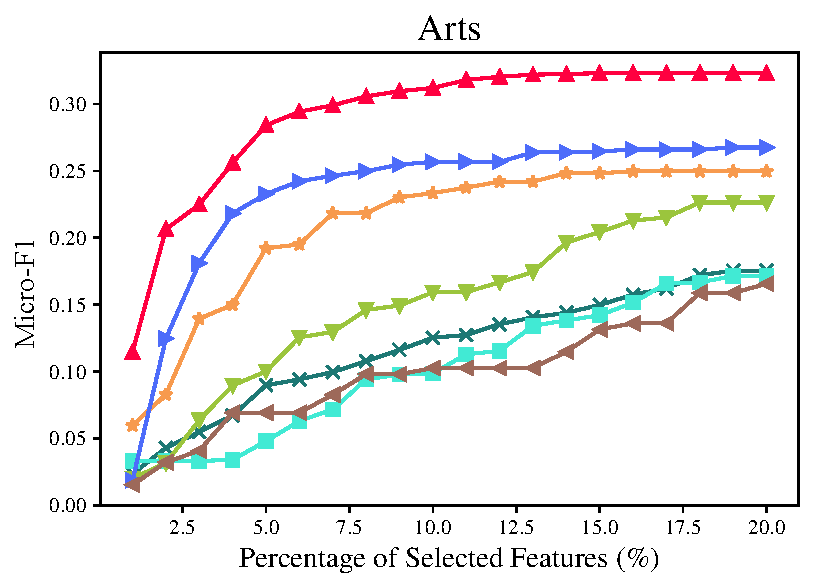
\includegraphics[width=0.43\textwidth]{figures/Micro/PSF(Arts).pdf}}
	{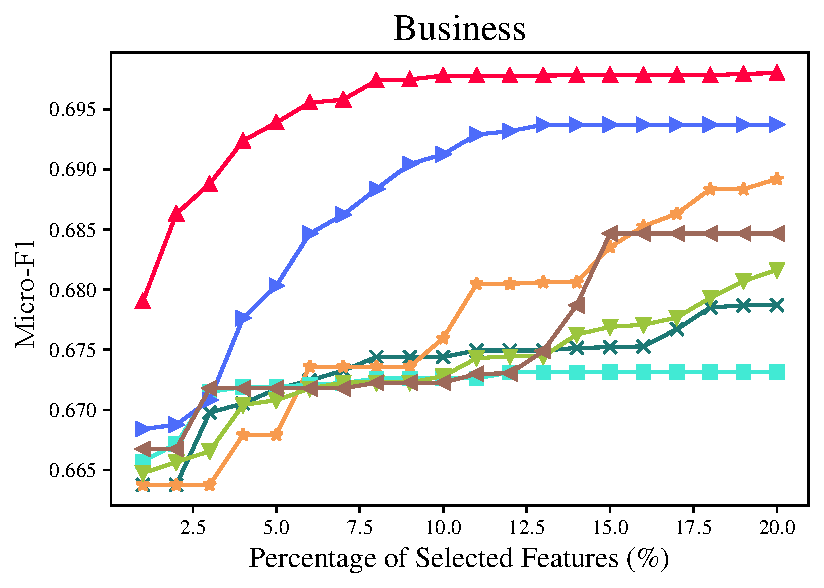
\includegraphics[width=0.43\textwidth]{figures/Micro/PSF(Business).pdf}}
	\\ 
	{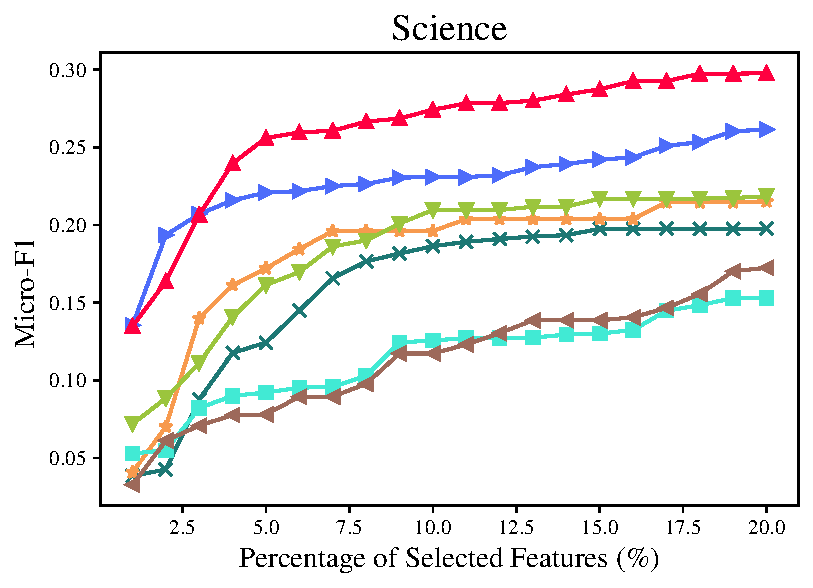
\includegraphics[width=0.43\textwidth]{figures/Micro/PSF(Science).pdf}}
	{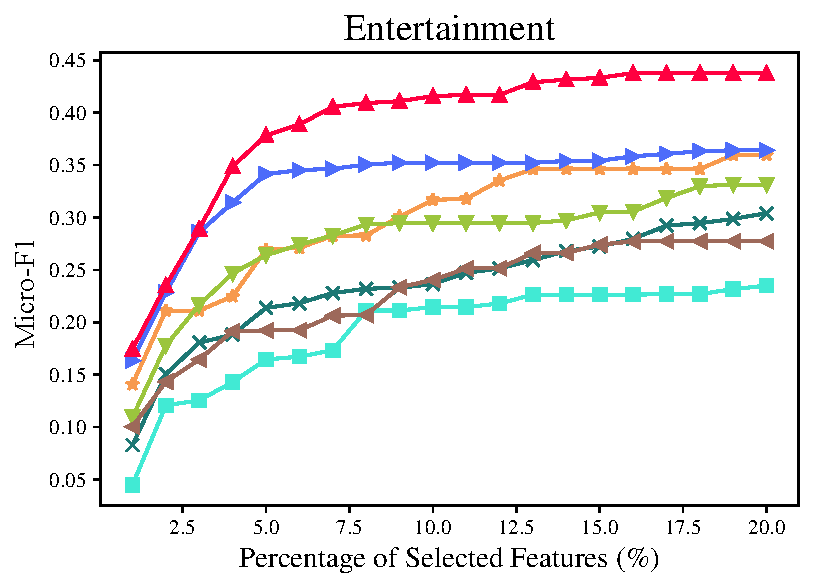
\includegraphics[width=0.43\textwidth]{figures/Micro/PSF(Entertainment).pdf}}
	{
\includegraphics[width=0.7\textwidth]{figures/Micro/FL.pdf}}
	\caption{نمودار درصد انتخاب ویژگی‌ها در معیار \lr{Micro-F1}}
	\label{fig:fmic}
\end{figure}
\begin{figure}
	\centering
	{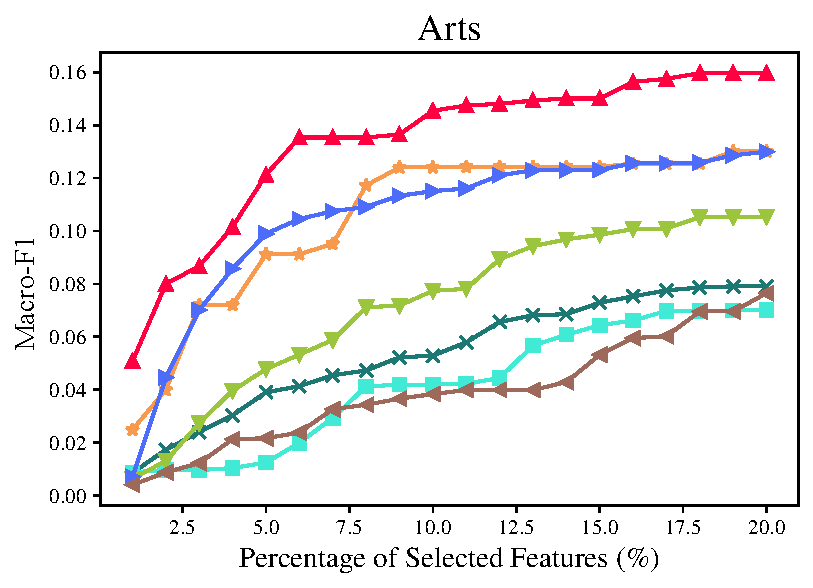
\includegraphics[width=0.43\textwidth]{figures/Macro/PSF(Arts).pdf}}
	{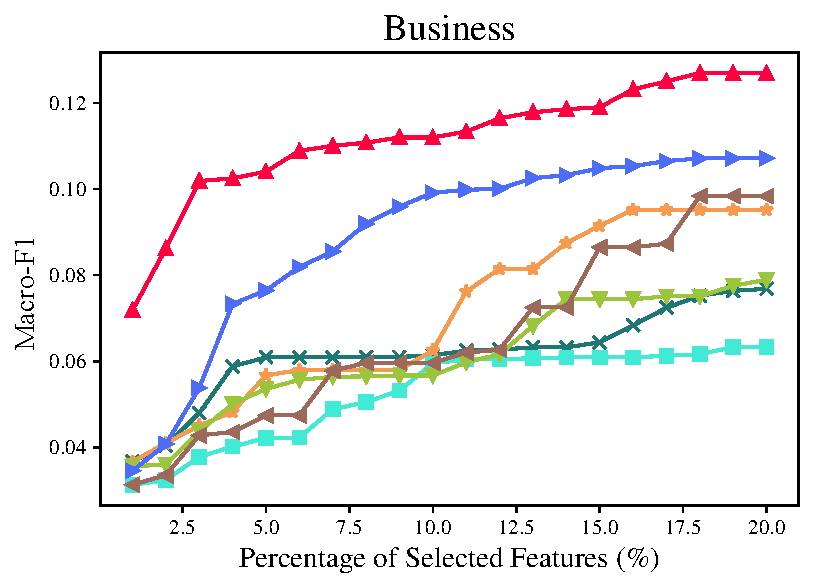
\includegraphics[width=0.43\textwidth]{figures/Macro/PSF(Business).pdf}}
	\\
	{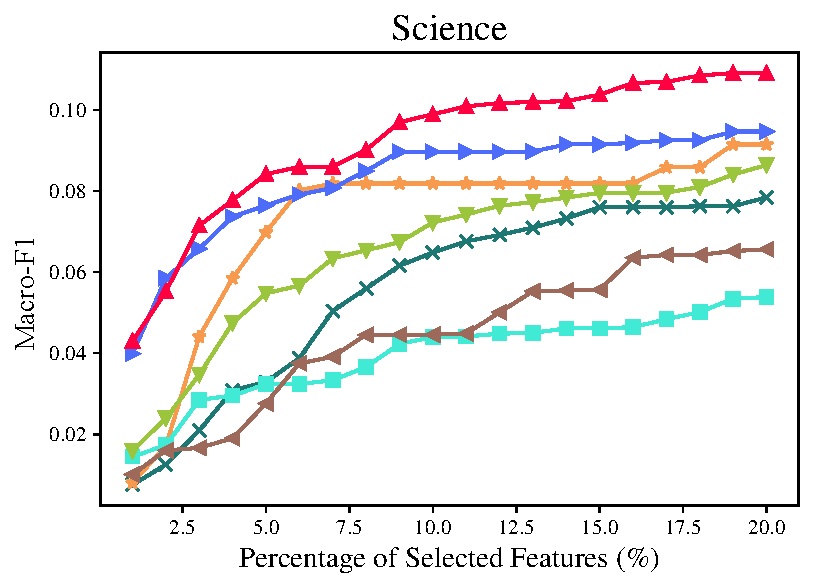
\includegraphics[width=0.43\textwidth]{figures/Macro/PSF(Science).pdf}}
	{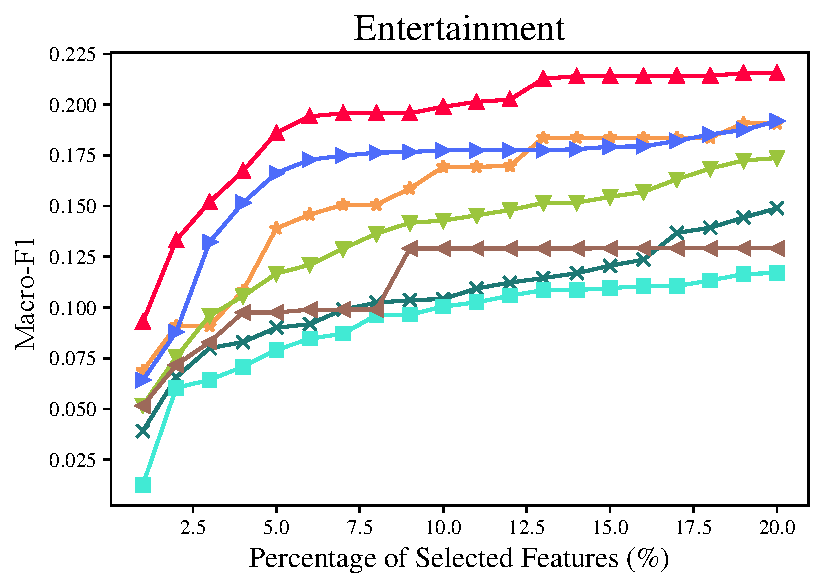
\includegraphics[width=0.43\textwidth]{figures/Macro/PSF(Entertainment).pdf}}
	{
\includegraphics[width=0.7\textwidth]{figures/Micro/FL.pdf}}
	\caption{نمودار درصد انتخاب ویژگی‌ها در معیار \lr{Macro-F1} }
	\label{fig:fmac}
\end{figure}
\begin{figure}
	\centering
	{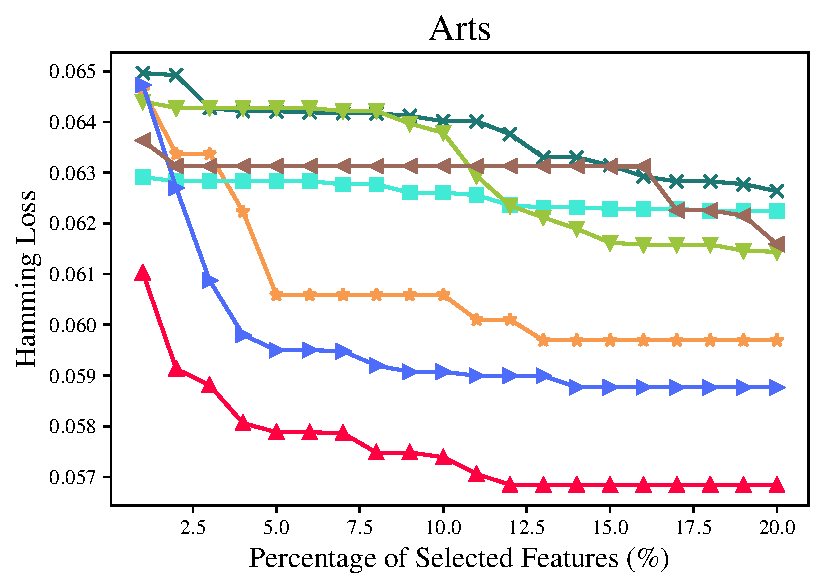
\includegraphics[width=0.43\textwidth]{figures/Hamming Loss/PSF(Arts).pdf}}
	{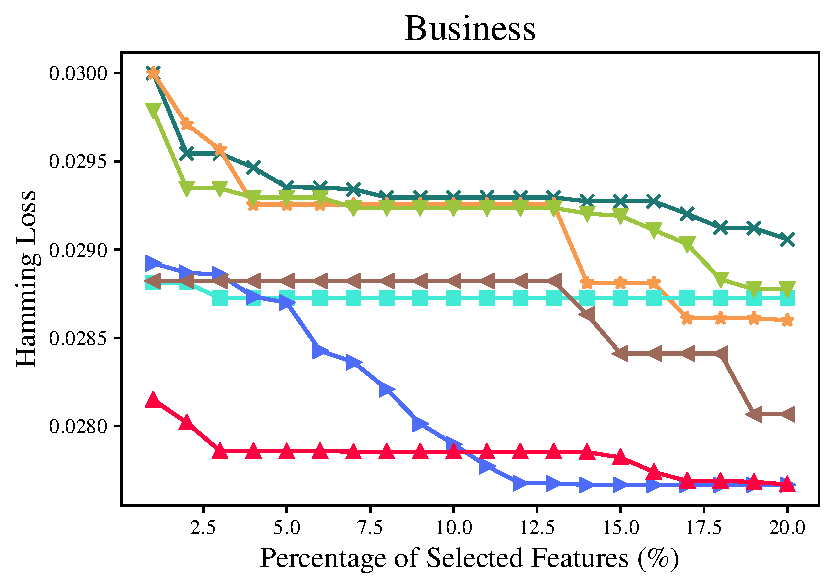
\includegraphics[width=0.43\textwidth]{figures/Hamming Loss/PSF(Business).pdf}}
	\\
	{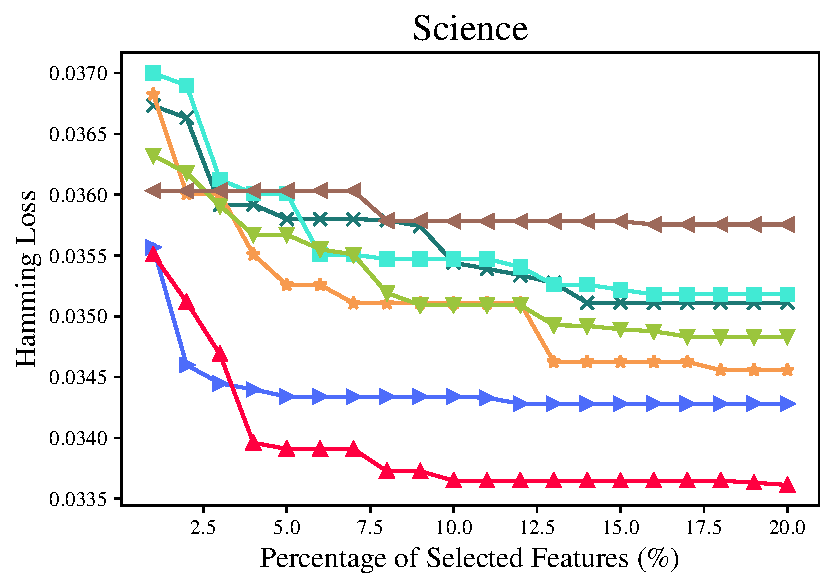
\includegraphics[width=0.43\textwidth]{figures/Hamming Loss/PSF(Science).pdf}}
	{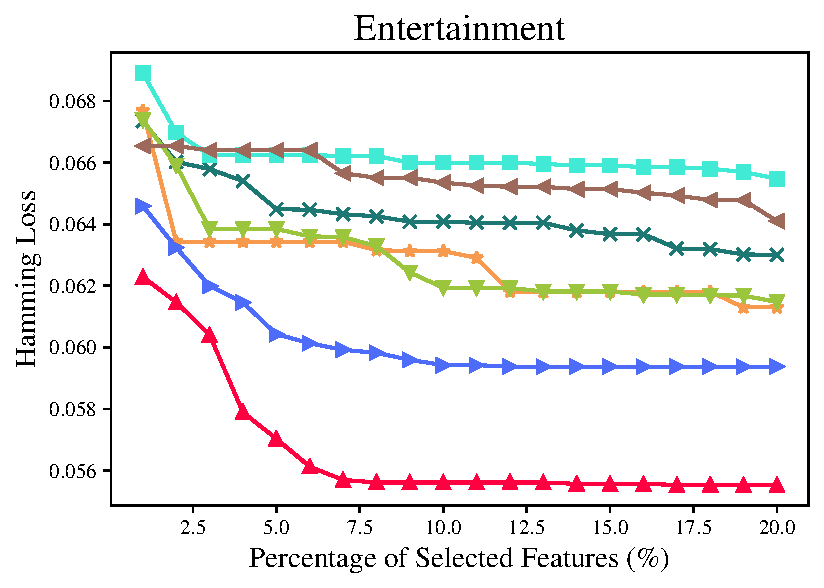
\includegraphics[width=0.43\textwidth]{figures/Hamming Loss/PSF(Entertainment).pdf}}
	{
\includegraphics[width=0.7\textwidth]{figures/Micro/FL.pdf}}
	\caption{نمودار درصد انتخاب ویژگی‌ها در معیار \lr{Hamming Loss} }
	\label{fig:fhml}
\end{figure}
\begin{figure}
	\centering
	{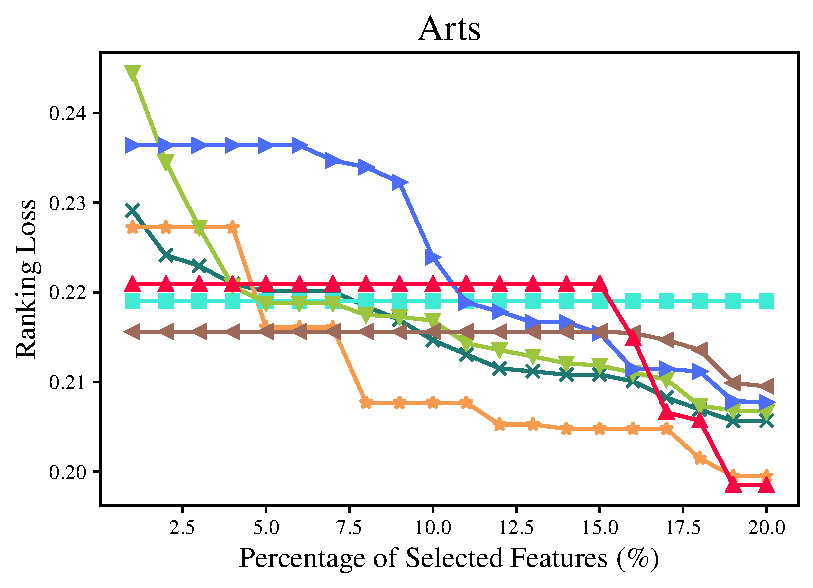
\includegraphics[width=0.43\textwidth]{figures/Ranking Loss/PSF(Arts).pdf}}
	{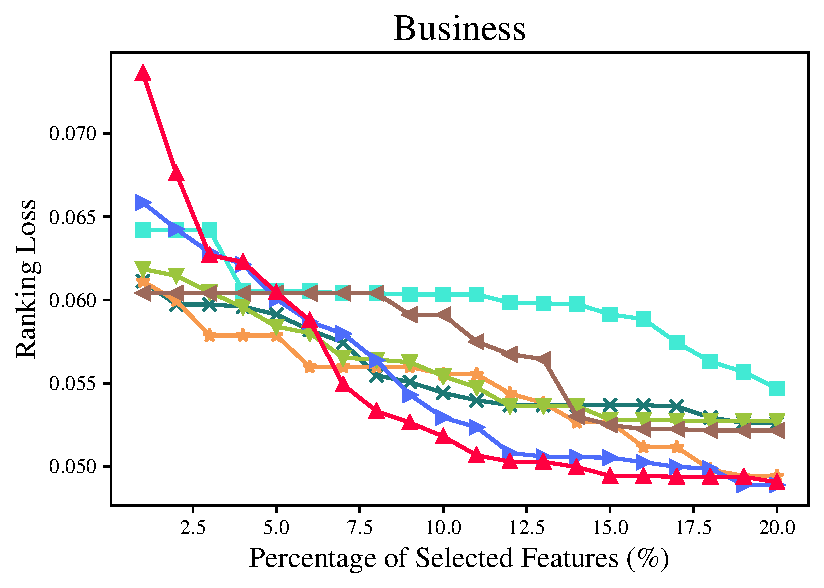
\includegraphics[width=0.43\textwidth]{figures/Ranking Loss/PSF(Business).pdf}}
	\\
	{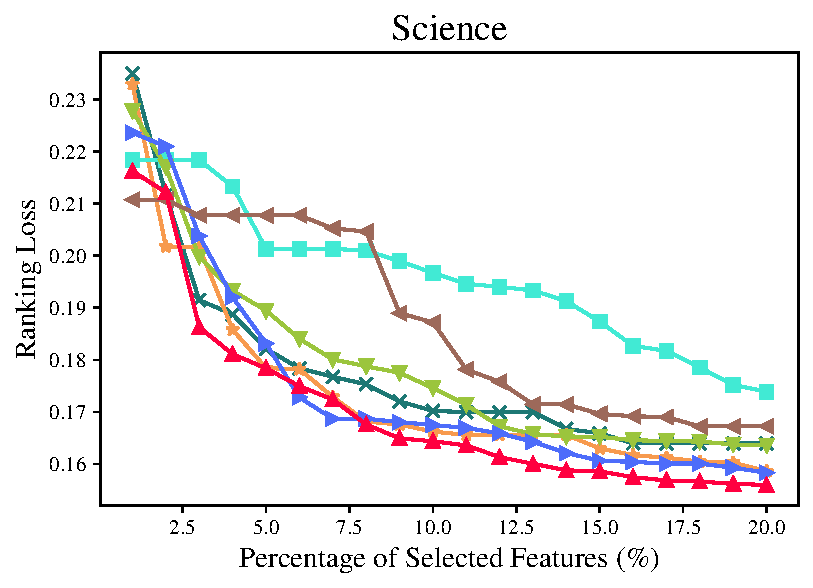
\includegraphics[width=0.43\textwidth]{figures/Ranking Loss/PSF(Science).pdf}}
	{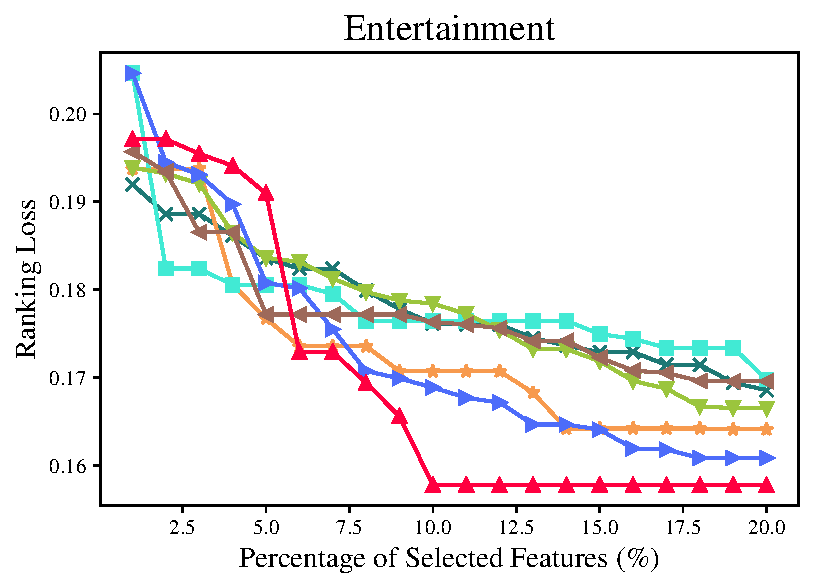
\includegraphics[width=0.43\textwidth]{figures/Ranking Loss/PSF(Entertainment).pdf}}
	{
\includegraphics[width=0.7\textwidth]{figures/Micro/FL.pdf}}
	\caption{\BNazTTN نمودار درصد انتخاب ویژگی‌ها در معیار \lr{Ranking Loss} }
	\label{fig:frnl}
\end{figure}
\section{تجزیه‌و‌تحلیل پارامترها}
در این بخش، تأثیر پارامترها، از جمله پارامتر منظم‌ساز گراف $\lambda_1$، پارامتر همبستگی برچسب سراسری و محلی $\lambda_2$، و پارامتر خلوتی $\lambda_3$ را تحلیل می‌کنیم. شکل‌های \ref{fig:P3D-MICMAC} و \ref{fig:PD3-HMLRNL} ‎\lr{Micro-F1}‎، ‎\lr{Macro-F1}‎، ‎\lr{Hamming Loss} و \lr{Ranking Loss } روش ما را با شش مجموعه‌داده $\lambda_1$، $\lambda_2،$ و $\lambda_3$ نشان می‌دهند. این شکل‌ها به‌صورت سه‌بعدی ترسیم شده‌اند، یعنی سه محور مربوط به $\lambda_1$، $\lambda_2$ و $\lambda_3$ است \cite{SALAHIAN2023119051}.

\begin{itemize}
	\item \subsubsection{ پارامتر $\lambda_1$}
	این پارامتر اثربخشی منظم‌ساز ‌خمینه فضای نمونه در مدل را کنترل  می‌کند. در این تحلیل پارامتر، مقادیر موجود در مجموعه
	\{100، 10، 1، 0/1، 0/01، 0\}
	برای پارامتر $\lambda_1$ در همه مجموعه‌های داده انتخاب شده‌اند. از شکل‌های \ref{fig:P3D-MICMAC}‎ و \ref{fig:PD3-HMLRNL} می‌توان نتیجه گرفت که مقدار بهینه برای این پارامتر معمولاً کمتر از ۱ است.
\end{itemize}
\begin{itemize}
	\item	\subsubsection{ پارامتر $\lambda_2$}
	این پارامتر اثربخشی همبستگی برچسب سراسری و محلی مدل را نشان می‌دهد و مقادیر تحلیل‌شده برای پارامتر $\lambda_2$
	\{0/1، 0/01، 0/001، \textsuperscript{6-}10، \textsuperscript{12-}10، 0\}
	هستند. همان‌طور که در شکل‌های \ref{fig:P3D-MICMAC} و \ref{fig:PD3-HMLRNL} مشاهده می‌کنیم، $\lambda_2$ با مقادیر کوچک معمولاً عملکرد بهتری را از نظر ‎\lr{Micro-F1}‎ و ‎\lr{Macro-F1}‎ نشان می‌دهد و با مقادیر بالا معمولاً از نظر معیارهای ‎\lr{Hamming Loss}‎ و ‎\lr{Coverage Error}‎ در چهار مجموعه‌داده عملکرد بهتری دارد. مقادیر نزدیک به صفر یا مقادیر بسیار بزرگ برای این پارامتر ممکن است عملکرد نسبتاً خوبی نداشته باشند.
\end{itemize}

\begin{itemize}
	\item	\subsubsection{ پارامتر $\lambda_3$}
	عبارت منظم‌ساز خلوت در ‎\lr{MLFS-GLOCAL}‎ توسط $\lambda_3$ کنترل می‌شود.  برای ‎پارامتر  $\lambda_3$‎
	محدوده مقادیر
	%\{0، 0.001، 0.1، 0.5، 1، 10\}
	\{10، 0/5، 0/1، 0/001، 0\}
	است. نتایج نشان می‌دهد که $\lambda_3$ یک کمیت ظریف است که معمولاً نیاز به تنظیم دقیق دارد. نتایج نشان می‌دهد که انتخاب مقادیر زیر 1 برای این پارامتر بهتر است.
\end{itemize}

\begin{figure}
	\centering
	\mysubfig{figures/Parameters3D/Health_Mic2.pdf}{Health}
	\mysubfig{figures/Parameters3D/Reference_Mic2.pdf}{Reference}
	\mysubfig{figures/Parameters3D/Society_Mic2.pdf}{Society}
	\\[0.5cm]
	\mysubfig{figures/Parameters3D/Health_Mac2.pdf}{Health}
	\mysubfig{figures/Parameters3D/Reference_Mac2.pdf}{Reference}
	\mysubfig{figures/Parameters3D/Society_Mac2.pdf}{Society}
	\\[0.3cm]
	\caption{تجزیه و تحلیل پارامترهای $\alpha$ و $\beta$ در مدل پیشنهادی }
	\label{fig:P3D-MICMAC}
\end{figure}
\begin{figure}
	\centering
	\mysubfig{figures/Parameters3D/Health_HML2.pdf}{Health}
	\mysubfig{figures/Parameters3D/Reference_HML2.pdf}{Reference}
	\mysubfig{figures/Parameters3D/Society_HML2.pdf}{Society}
	\\[0.5cm]
	\mysubfig{figures/Parameters3D/Health_RNL2.pdf}{Health}
	\mysubfig{figures/Parameters3D/Reference_RNL2.pdf}{Reference}
	\mysubfig{figures/Parameters3D/Society_RNL2.pdf}{Society}
	\\[0.3cm]
	\caption{تجزیه و تحلیل پارامترهای $\alpha$ و $\beta$ در مدل پیشنهادی }
	\label{fig:PD3-HMLRNL}
\end{figure}


%\begin{figure}
%	\centering
%	\captionsetup[subfigure]{position=top}
%	\subfloat[]{{\includegraphics[trim={0 1cm 0 0},clip,width=12cm]{figures/AUC Different Attack.eps}}}
%	\\
%	\subfloat[]{{\includegraphics[trim={9.25cm 2cm 0 0},clip,width=12.1cm]{figures/Precision Different Attack.eps}}}
%	\\
%	\includegraphics[height=0.7cm]{figures/Dataset name for different attack-pdf-crop.pdf}
%	\caption{نتایج ارزیابی در برابر حملات مختلف مهاجم}
%	\label{fig:4}
%\end{figure}


%\begin{figure}
%	\centering
%	\captionsetup[subfigure]{position=top}
%	\subfloat[C.elegans]{{\includegraphics[trim={0 0 0 1cm},clip,width=5cm]{figures/AUCCelegansneuralRemoveLink.eps}}}\quad
%	\subfloat[YeastL]{{\includegraphics[trim={0 0 0 1cm},clip,width=5cm]{figures/AUCYeastLRemoveLink.eps}}}
%	\\
%	\subfloat[ODLIS]{{\includegraphics[trim={0 0 0 1cm},clip,width=5cm]{figures/AUCODLISRemoveLink.eps}}}\quad
%	\subfloat[OpenFlights]{{\includegraphics[trim={0 0 0 1cm},clip,width=5cm]{figures/AUCOpenflightsRemoveLink.eps}}}
%	\\
%	\subfloat[SciMet]{{\includegraphics[trim={0 0 0 1cm},clip,width=5cm]{figures/AUCSciMetRemoveLink.eps}}}\quad
%	\subfloat[Power-US]{{\includegraphics[trim={0 0 0 1cm},clip,width=5cm]{figures/AUCPowerUSRemoveLink.eps}}}
%	\\
%	\includegraphics[height=0.47cm]{figures/Name-removed link-pdf-crop.pdf}
%	\caption{میزبه‌صورت مقاوم پذیری روش ‎\lr{LPANMF}‎ }
%	\label{fig:3}
%\end{figure}

\section{تحلیل همگرایی }
در این بخش، ما رفتار همگرایی\LTRfootnote{Convergence} مدل پیشنهادی \eqref{eq:BeOpt} را با انجام آزمایش‌هایی بر روی چهار مجموعه‌داده 
‎\lr{Arts}، \lr{Corel5k}، \lr{Health} و \lr{Reference}
ارزیابی می‌کنیم.
‎ الگوریتم \ref{alg:algorithm} را برای هر مجموعه‌داده با 600 تکرار اجرا می‌کنیم. مقدار تابع هدف را در برابر تعداد تکرارها در شکل \ref{fig:7} رسم کرده‌ایم تا نشان دهیم چگونه روش ما‌ همگرا می‌شود. همان‌طور که از شکل \ref{fig:7} مشاهده می‌شود، مقدار تابع هدف به سرعت و به‌طور پیوسته در تکرارهای اولیه کاهش می‌یابد، که نشان می‌دهد روش ما به سرعت به یک راه‌حل بهینه نزدیک می‌شود. در تکرارهای بعدی، مقدار تابع هدف بسیار کم تغییر می‌کند، و این نشان می‌دهد روش ما به یک راه‌حل تقریباً بهینه رسیده است. این بیانگر این می‌باشد که روش ارائه‌شده عملکرد همگرایی سریع و پایداری دارد.
\begin{figure}
	\centering
	\begin{minipage}[b]{0.48\textwidth}
		\centering
		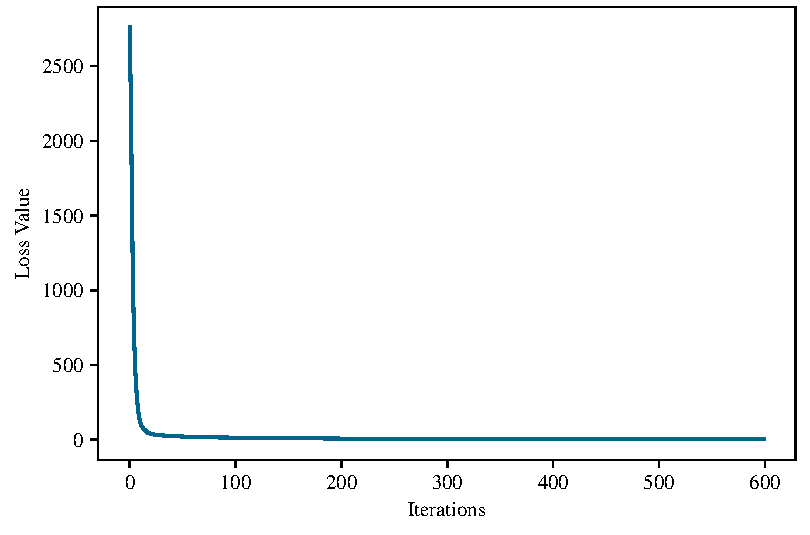
\includegraphics[width=\textwidth]{figures/Convergence/Convergence(Arts).pdf}
		\caption*{\centering Arts}
	\end{minipage}\hfill
	\begin{minipage}[b]{0.48\textwidth}
		\centering
		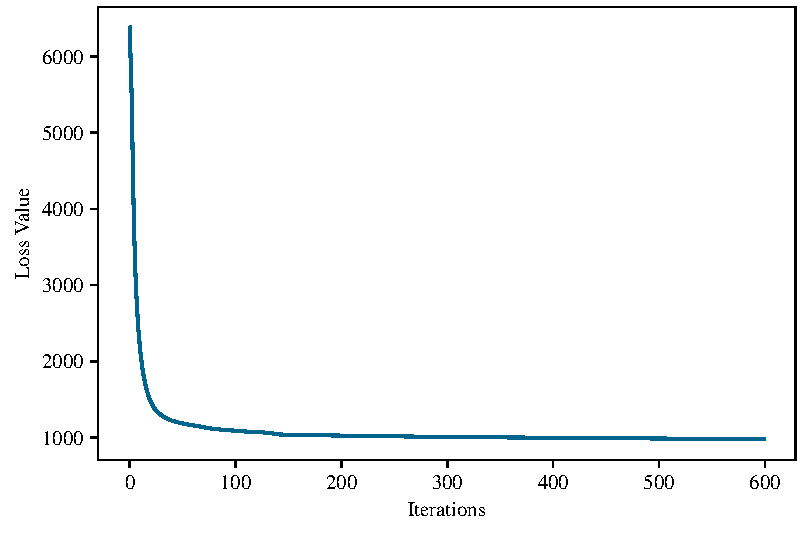
\includegraphics[width=\textwidth]{figures/Convergence/Convergence(Corel5k).pdf}
		\caption*{\centering Corel5k}
	\end{minipage}
	\\[0.5cm]
	\begin{minipage}[b]{0.48\textwidth}
		\centering
		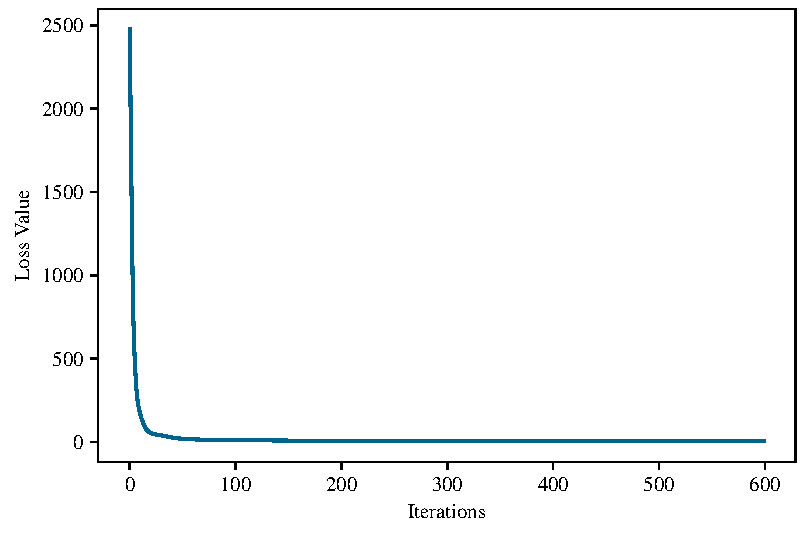
\includegraphics[width=\textwidth]{figures/Convergence/Convergence(Health).pdf}
		\caption*{\centering Health}
	\end{minipage}\hfill
	\begin{minipage}[b]{0.48\textwidth}
		\centering
		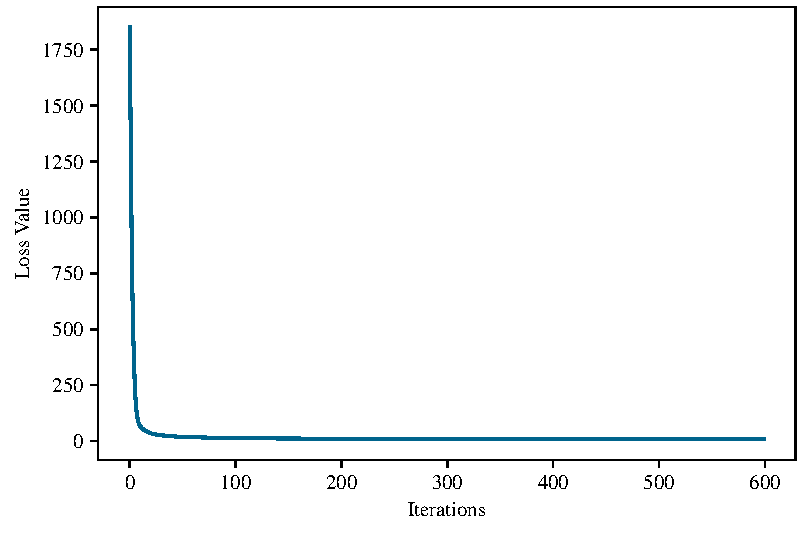
\includegraphics[width=\textwidth]{figures/Convergence/Convergence(Reference).pdf}
		\caption*{\centering Reference}
	\end{minipage}
	\caption{همگرایی مدل پیشنهادی \lr{(MLFS-GLOCAL)}}‎
	\label{fig:7}
\end{figure}
